\boldmath

\chapter{Modellazione del Sistema nell'ambiente Simulink}

    \noindent In questo capitolo esploreremo l'ambiente Simulink di MATLAB, uno strumento avanzato per la modellazione, la simulazione e l'analisi di sistemi dinamici. Simulink consente di creare modelli grafici dei sistemi utilizzando un'interfaccia intuitiva a blocchi, facilitando la rappresentazione e la comprensione delle interazioni tra i vari componenti del sistema. Attraverso esempi pratici e casi di studio, illustreremo come costruire modelli accurati, simulare il comportamento del sistema e analizzare i risultati per ottimizzare le prestazioni. Particolare attenzione sarà dedicata a Stateflow, un modulo di Simulink specializzato nella gestione di logiche basate su stati, condizioni decisionali e comportamenti che cambiano nel tempo.

    \section{Gate Chart}
        In questa sezione esamineremo l'implementazione del modulo principale \textbf{Cancello}, che si occupa della movimentazione dello stesso, dell'attivazione e disattivazione dei LED, e della gestione dello stato di errore.

        \newpage
            
        \subsection{Variabili}
            Le variabili presenti all'interno del macrostato sono le seguenti:
            \begin{table}[H]
                \centering
                    \begin{tabular}{ | c | c | c | c |} 
                        \hline
                        \textbf{Tipo} & \textbf{Nome} & \textbf{Valore} & \textbf{Descrizione} \\
                        
                        \hline
                        local\_data & Var\_Inattivo & ON/OFF &  \makecell{Variabile utilizzata per segnalare \\ che lo stato Inattivo è attualmente attivo}\\
                        
                        \hline
                        local\_data & Var\_Chiuso & ON/OFF & \makecell{Variabile utilizzata per segnalare \\ che lo stato Chiuso è attualmente attivo} \\
                        
                        \hline
                        local\_data & Var\_Aperto & ON/OFF & \makecell{Variabile utilizzata per segnalare \\ che lo stato Aperto è attualmente attivo} \\
                        
                        \hline
                        local\_data & Var\_In\_Chiusura & ON/OFF & \makecell{Variabile utilizzata per segnalare \\ che lo stato In Chiusura è attualmente attivo} \\
                        
                        \hline
                        output\_data & LedG & ON/OFF & \makecell{Variabile utilizzata per l'attivazione del \\ LED verde in output} \\
                        
                        \hline
                        output\_data & LedR & ON/OFF & \makecell{Variabile utilizzata per l'attivazione del \\ LED Rosso in output} \\
                        
                        \hline
                        output\_data & LedY & ON/OFF & \makecell{Variabile utilizzata per l'attivazione del \\ LED Giallo in output} \\
                        
                        \hline
                        input\_data & P1 & ON/OFF & \makecell{Variabile utilizzata per \\ la segnalazione di un ostacolo} \\
                        
                        \hline
                        input\_data & P2 &ON/OFF & \makecell{Variabile utilizzata per \\ la segnalazione della chiusura del cancello} \\
                        
                        \hline
                        constant\_data & Blink\_Period & 2 & \makecell{Costante utilizzata per la durata del \\ blink del LED Giallo} \\
                        
                        \hline
                        local\_data & $T_L$ & [10, 120] & Contatore del tempo di lavoro \\
                        
                        \hline
                        local\_data & $T_C$ & [10, 120] & Contatore del tempo di chiusura \\
                        
                        \hline
                        constant\_data & ErrDur & 10 & \makecell{Costante utilizzata per la durata del \\ lampeggio del LED rosso} \\
                        
                        \hline
                        local\_event & buttonpressed1 & TRUE/FALSE & Evento per la pressione del pulsante B1 \\
                        
                        \hline
                    \end{tabular}
                \caption{Tabella variabili Cancello}
            \end{table}

        \subsection{Stati e Funzionamento}
            Il macrostato \textbf{Cancello} presenta i seguenti stati e macrostati:
                
            \begin{itemize}
                \item \textbf{Inattivo}
                    
                \item \textbf{Chiusura}  
                    \begin{itemize}    
                        \item In Chiusura  
                            \begin{itemize}
                                \item Blink\_COff
                                    
                                \item Blink\_COn
                            \end{itemize}
                        
                        \item Chiuso
                        
                        \item Errore
                            \begin{itemize}
                                \item In errore
                                    
                                    \begin{itemize}
                                        \item Blink\_EOff
                                            
                                        \item Blink\_EOn
                                    \end{itemize}
                                
                                \item Led\_Rosso\_Errore
                            \end{itemize}
                    \end{itemize}
                    
                \item \textbf{Apertura}
                    \begin{itemize}
                        \item In Apertura
                            \begin{itemize}
                                \item Blink\_AOff
                                    
                                \item Blink\_AOn 
                            \end{itemize}
                            
                        \item Aperto
                            
                        \item Aperto\_Con\_Ostacolo
                    \end{itemize}
            \end{itemize}
                
            \begin{figure}[H]
                \centering
                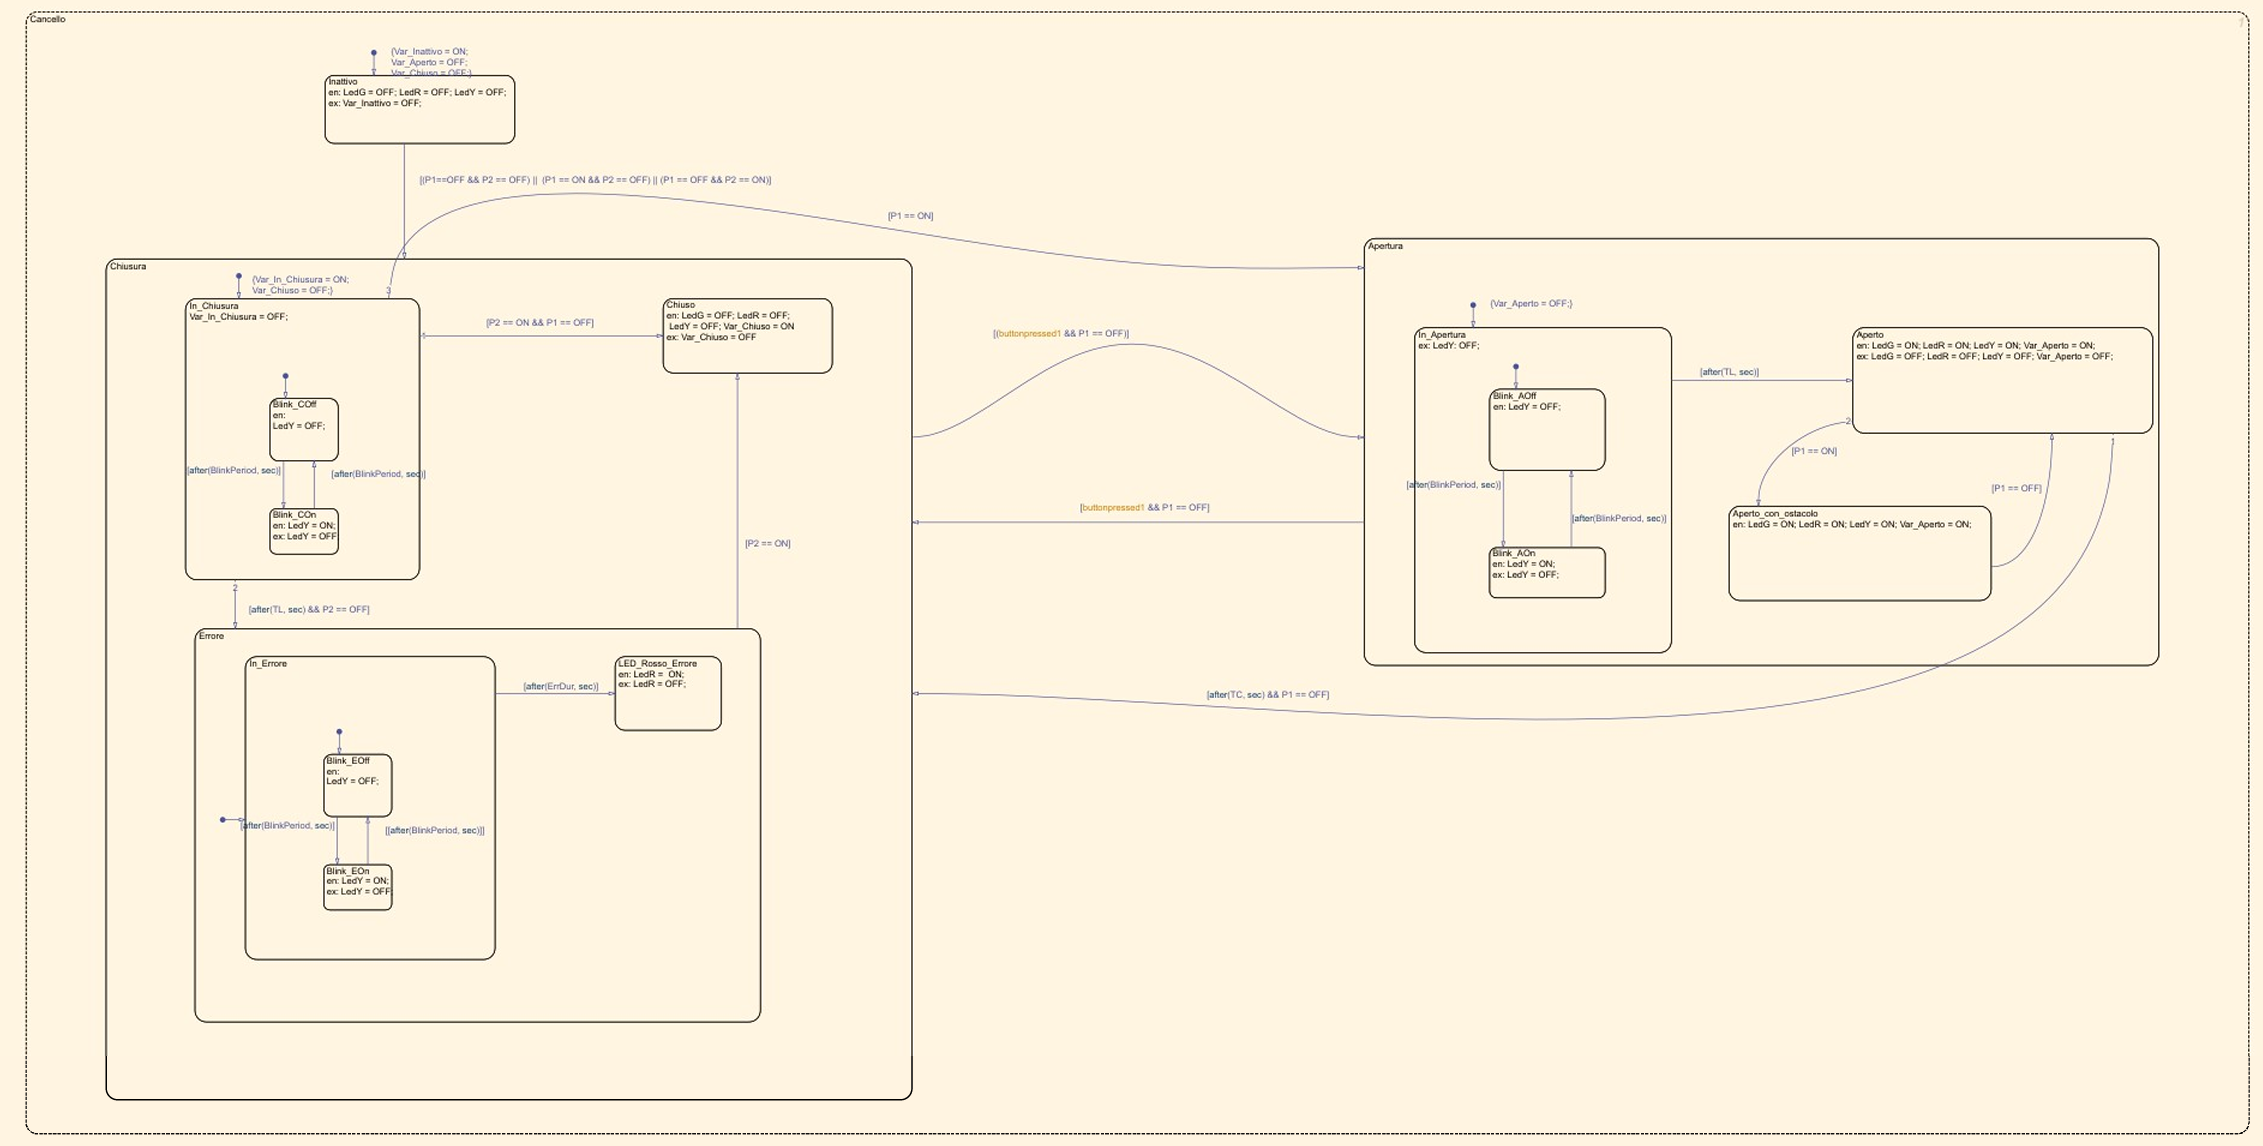
\includegraphics[width=0.9\textwidth]{figures/gate.png}
                \caption{Stato Cancello}
                \label{gate}
            \end{figure}

            \noindent Proseguiamo ora descrivendo il funzionamento dell'intero macrostato \textbf{Cancello}
        
            \begin{enumerate}
                \item All'avvio del sistema lo stato è impostato come \textbf{Inattivo}, inizializza le tre variabili \textit{Var\_Inattivo}, \textit{Var\_Aperto} e \textit{Var\_Chiuso} e si occupa di spegnere tutti i LED.
                Quando si esce da codesto stato, si pone \textit{Var\_Inattivo} ad OFF.
                La condizione di uscita prevede che si vada nello stato \textbf{Chiusura} se e solo se i due sensori di presenza non sono contemporaneamente e inizialmente attivi.
                
                \item All'interno del macrostato \textbf{Chiusura}, lo stato iniziale è \textbf{In\_Chiusura}, in cui viene inizializzata la variabile \textit{Var\_In\_Chiusura} ad ON, mentre la variabile \textit{Var\_Chiuso} viene posta ad OFF.
                Inoltre, nel macrostato \textbf{In\_Chiusura}, avviene il blink del LED giallo grazie all'alternarsi degli stati sottostanti con periodo di 2 secondi. \\
                Le transizioni in uscita da questo stato sono:
            
                \begin{itemize}
                    \item Se si attiva il sensore di presenza P2 di chiusura del cancello, ed il sensore P1 risulta spento (non rilevando dunque ostacoli), si entra nello stato \textbf{Chiuso}, nel quale vengono spenti tutti i LED e viene attivata la variabile \textit{Var\_Chiuso}
                    
                    \item Se scade il timer riguardante il tempo di lavoro \textbf{$T_L$} senza conseguente attivazione del sensore di presenza P2, si entra nello stato \textbf{Errore}, nel quale si accende il LED rosso se e solo se vi si permane  per ulteriori 10 secondi. Si esce da questo stato solo se ritorna attivo il sensore di presenza P2
                    
                    \item Se invece, si attiva il sensore di presenza P1 che rileva un ostacolo durante la chiusura, si entra nel macrostato \textbf{Apertura}
                \end{itemize}
            
                \item All'interno del macrostato \textbf{Apertura}, lo stato iniziale è quello \textbf{In\_Apertura}, nel quale viene effettuato il blink del LED giallo grazie all'alternarsi degli stati sottostanti con periodo di 2 secondi.
                Da questo stato si esce solo quando scade il tempo di lavoro \textbf{$T_L$} per poi passare allo stato \textbf{Aperto}.
                
                \item In questo stato vengono accesi tutti i LED per segnalare la corretta apertura del cancello e viene posta ad ON la variabile \textit{Var\_Aperto}. In uscita da questo stato invece, i LED verranno spenti ponendo ad OFF la variabile \textit{Var\_Aperto}. \\
                Le possibili transizioni per uscire da questo stato sono:
                
                \begin{itemize}
                    \item Se viene rilevato un ostacolo si entra nello stato \textbf{Aperto\_Con\_Ostacolo} nel quale vengono riaccesi tutti i LED e l'unica transizione possibile per uscire da questo stato è quando non viene più rilevato.
                    Questa funzionalità è stata implementata per azzerare il timer di chiusura ogni volta che un ostacolo viene rilevato
                    
                    \item Se scade il tempo di chiusura e non viene rilevato alcun ostacolo, allora si entra nel macrostato \textbf{Chiusura}, il quale avvia il processo di chiusura del cancello
                \end{itemize}
                
                \item Sia nel macrostato \textbf{Chiusura} che \textbf{Apertura}, la transizione di uscita è identica, nella quale viene premuto il pulsante B1 e non vi sono ostacoli rilevati dal sensore di presenza P1.
            \end{enumerate}


    \section{Tuning Charts}
        In questa sezione analizzeremo l'implementazione dei due moduli utilizzati per le regolazioni, \textbf{Regolazione\_Tempo\_Chiusura} e \textbf{Regolazione\_Tempo\_Lavoro}.
        Essi permettono di regolare le due variabili \textbf{$T_C$} e \textbf{$T_L$} attraverso la pressione dei pulsanti \textbf{$B2$} e \textbf{$B3$} rispettivamente.

        \subsection{Variabili}
            Le variabili presenti all'interno dei due macrostati sono le seguenti:
            
            \begin{table}[H]
                \centering
                    \begin{tabular}{ | c | c | c | c |} 
                        \hline
                        
                        \textbf{Tipo} & \textbf{Nome} & \textbf{Valore} & \textbf{Descrizione} \\ 
                        \hline
                        
                        input\_data & $T_L$ & [10, 120] & Contatore del tempo di lavoro \\ 
                        \hline
                        
                        input\_data & Var\_Chiuso & ON/OFF & \makecell{Variabile utilizzata per segnalare \\ che lo stato Chiuso è attualmente attivo} \\ 
                        \hline
                        
                        local\_event & buttonpressed3 & TRUE/FALSE & Evento per la pressione del pulsante B3 \\ 
                        \hline
                        
                        input\_data & $T_C$ & [10, 120] & Contatore del tempo di chiusura \\ 
                        \hline
                        
                        local\_event & buttonpressed2 & TRUE/FALSE & Evento per la pressione del pulsante B2 \\ 
                        \hline
                    \end{tabular}
                \caption{Tabella variabili Tuning}
            \end{table}

        \subsection{Stati e Funzionamento}
            \noindent I due macrostati presentano i seguenti stati al loro interno:
            
            \begin{itemize}
                \item \textbf{Regolazione\_Tempo\_Lavoro}
                \begin{itemize}
                    \item \textit{Tempo\_Lavoro}
                    \item \textit{Aggiunta\_Tempo\_Lavoro}
                \end{itemize}

                \item \textbf{Regolazione\_Tempo\_Lavoro}
                \begin{itemize}
                    \item \textit{Tempo\_Chiusura}
                    \item \textit{Aggiunta\_Tempo\_Chiusura}
                \end{itemize}
            \end{itemize}

            \begin{figure}[H]
                \centering
                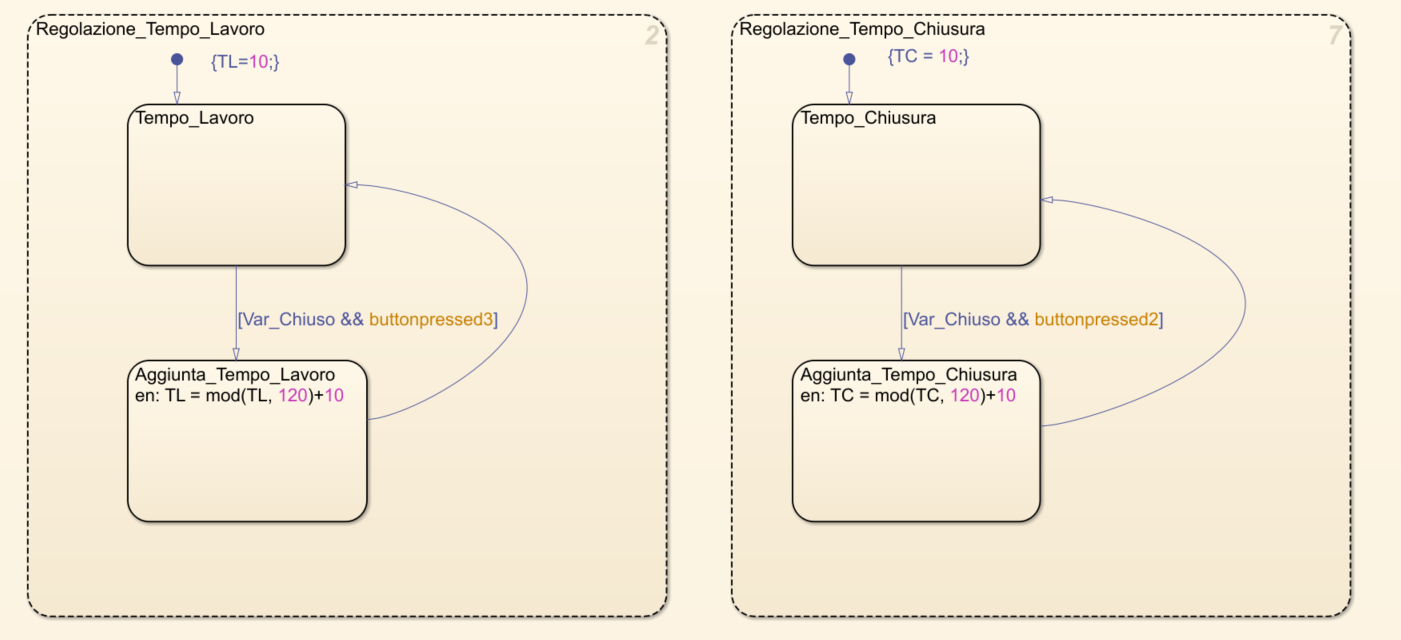
\includegraphics[width=0.9\textwidth]{figures/tuning.png}
                \caption{Stati Regolazioni}
                \label{tuning}
            \end{figure}

            \noindent Proseguiamo ora analizzando il funzionamento di un singolo macrostato \textbf{(Regolazione\_Tempo\_Chiusura)}, essendo l'altro identico per costruzione:

            \begin{enumerate}
                \item Si parte dallo stato \textbf{Tempo\_Chiusura} nel quale la variabile \textbf{$T_C$} viene inizializzata al valore 10 (secondi).
                
                \item In seguito, se ci troviamo nello stato \textbf{Chiuso} e parallelamente viene rilevata la pressione del pulsante \textbf{B2} allora, ci spostiamo nello stato \textbf{Aggiunta\_Tempo\_Chiusura} nel quale la variabile $T_C$ viene incrementata di 10 (secondi).
                
                \item Una volta avvenuto l'incremento, si ritorna nello stato iniziale \textbf{Tempo\_Chiusura} nel quale si resta in attesa delle condizioni tali per cui si possono effettuare gli ulteriori incrementi.
            \end{enumerate}


    \section{Obstacle Chart}
        In questa sezione analizzeremo l'implementazione del macrostato \textbf{Ostacolo}, il quale consente la gestione del sistema in caso di rilevazione dello stesso. Esso permette il lampeggio del LED verde in output, nel caso il sensore di presenza \textbf{P1} si attivi.

        \subsection{Variabili}
            Le variabili all'interno del macrostato sono le seguenti:
            
            \begin{table}[H]
                \centering
                    \begin{tabular}{ | c | c | c | c |} 
                        \hline
                        
                        \textbf{Tipo} & \textbf{Nome} & \textbf{Valore} & \textbf{Descrizione} \\ 
                        \hline
                        
                        constant\_data & GreenDur & 30 & \makecell{Costante utilizzata per la durata del \\ lampeggio del LED verde} \\ 
                        \hline
                        
                        input\_data & Var\_Chiuso & ON/OFF & \makecell{Variabile utilizzata per segnalare \\ che lo stato Chiuso è attualmente attivo} \\ 
                        \hline
                        
                        input\_data & Var\_Inattivo & ON/OFF & \makecell{Variabile utilizzata per segnalare \\ che lo stato Inattivo è attualmente attivo} \\ 
                        \hline
                        
                        input\_data & Var\_Aperto & ON/OFF & \makecell{Variabile utilizzata per segnalare \\ che lo stato Aperto è attualmente attivo} \\ 
                        \hline
                        
                        local\_event & buttonpressed1 & TRUE/FALSE & Evento per la pressione del pulsante B1 \\ 
                        \hline
                        
                        constant\_data & BlinkPeriod2 & 1 & \makecell{Costante utilizzata per la durata del \\ blink del LED verde} \\ 
                        \hline
                        
                        input\_data & P1 & ON/OFF & \makecell{Variabile utilizzata per \\ la segnalazione di un ostacolo} \\ 
                        \hline
                        
                        output\_data & LedG & ON/OFF & \makecell{Variabile utilizzata per l'attivazione del \\ LED verde in output} \\ 
                        \hline
                    \end{tabular}
                \caption{Tabella variabili Ostacolo}
            \end{table}

        \subsection{Stati e Funzionamento}
            Il macrostato \textbf{Ostacolo} presenta i seguenti stati al suo interno:
            
            \begin{itemize}
                \item \textbf{Fermo}
                
                \item \textbf{Ostacolo\_Presente}
                
                \item \textbf{Blink\_OOff}
                
                \item \textbf{Blink\_OOn}
                
                \item \textbf{Aperto\_Con\_Ostacolo\_Led}
            \end{itemize}

            \begin{figure}[H]
                \centering
                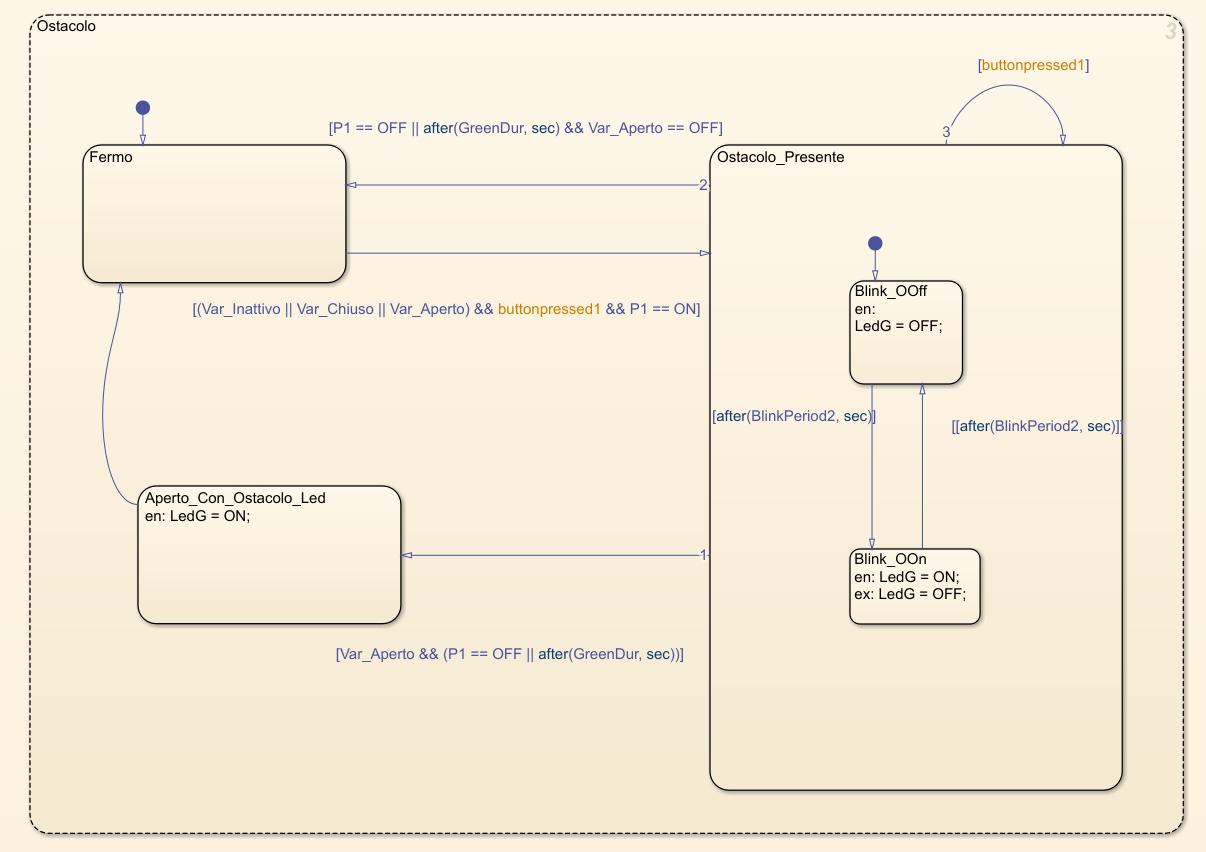
\includegraphics[width=0.9\textwidth]{figures/obstacle.png}
                \caption{Stato Ostacolo}
                \label{obstacle}
            \end{figure}

            \noindent Proseguiamo ora descrivendo il funzionamento dell'intero macrostato \textbf{Ostacolo}:
            
            \begin{enumerate}
                \item All'attivazione del sistema, si entra nello stato \textbf{Fermo} (che rappresenta uno stato di \textit{Idle}) dal quale si esce solo quando ci si trova  o nello stato \textbf{Inattivo} o nello stato \textbf{Chiuso} o nello stato \textbf{Aperto} e al contempo il sensore di presenza \textbf{P1} è attivo con annessa rilevazione di pressione del pulsante \textbf{$B1$}.
                
                \item La transizione sopra citata, ci porta nello stato \textbf{Ostacolo\_Presente} nel quale viene effettuato il \textit{blink} del LED verde.
                Nel dettaglio, lo stato iniziale del blink è \textbf{Blink\_OOff} il quale si occupa di spegnere il LED verde, mentre lo stato \textbf{Blink\_OOn} si occupa di accenderlo.
                La transizione tra i due stati avviene in accordo alla scadenza di un timer, di durata pari a \textbf{Blink\_Period2}, ovvero 1 secondo.
                
                \item Dall'attuale stato, si esce quando si verifica una delle seguenti condizioni:
                
                    \begin{itemize}
                        \item Non viene più rilevato l'ostacolo poiché il sensore di presenza P1 si disattiva, oppure poiché scade il timer associato al lampeggio del LED.
                        In aggiunta a questi requisiti \textbf{Var\_Aperto} deve essere uguale ad OFF.
                        In questo caso, ritorniamo nello stato \textbf{Fermo}.
                        
                        \item Non viene più rilevato l'ostacolo poiché il sensore di presenza P1 si disattiva, oppure poiché scade il timer associato al lampeggio del LED, ma ci troviamo parallelamente nello stato \textbf{Aperto}, dunque, il nuovo stato diventa \textbf{Aperto\_Con\_Ostacolo\_Led} nel quale viene riattivato il LED verde dopo il lampeggio.
                        Infine si ritorna nello stato \textbf{Fermo}.
                        \item Si preme il pulsante B1 e si ritorna nello stato \textbf{Ostacolo\_Presente} in modo da resettare il timer di 30 secondi relativo al lampeggio del LED verde.
                    \end{itemize}
            \end{enumerate}


    \section{Buttons Charts}
        In questa sezione analizzeremo l'implementazione dei macrostati \textbf{Button}. Essi permettono di rilevare quando il pulsante è stato premuto consentendo l'attivazione dell'evento. 
        Vedremo prima l'implementazione del macrostato \textbf{Button1} e successivamente di \textbf{Button2} e \textbf{Button3} che sono identici per costruzione.

        \subsection{Variabili}
        Le variabili all'interno del macrostato \textbf{Button1} sono le seguenti:

            \begin{table}[H]
                \centering
                    \begin{tabular}{ | c | c | c | c |} 
                        \hline
                        \textbf{Tipo} & \textbf{Nome} & \textbf{Valore} & \textbf{Descrizione} \\ 
                        
                        \hline
                        input\_data & B1 & ON/OFF & \makecell{Variabile utilizzata per segnalare \\ la pressione del pulsante} \\ 
                        
                        \hline
                        local\_event & buttonpressed1 & TRUE/FALSE & Evento per la pressione del pulsante B1 \\ 
                        
                        \hline
                    \end{tabular}
                \caption{Tabella variabili Button1}
            \end{table}
            
            Le variabili all'interno dei macrostati \textbf{Button2} e \textbf{Button3} sono le seguenti:

            \begin{table}[H]
                \centering
                    \begin{tabular}{ | c | c | c | c |} 
                        \hline
                        \textbf{Tipo} & \textbf{Nome} & \textbf{Valore} & \textbf{Descrizione} \\ 
                        \hline
                        input\_data & B2 & ON/OFF & \makecell{Variabile utilizzata per segnalare \\ la pressione del pulsante} \\ 
                        \hline
                        local\_event & buttonpressed2 & TRUE/FALSE & Evento per la pressione del pulsante B2 \\ 
                        \hline
                        input\_data & B3 & ON/OFF & \makecell{Variabile utilizzata per segnalare \\ la pressione del pulsante} \\ 
                        \hline
                        local\_event & buttonpressed3 & TRUE/FALSE & Evento per la pressione del pulsante B3 \\ 
                        \hline
                    \end{tabular}
                \caption{Tabella variabili Button2 e Button3}
            \end{table}

        \subsection{Stati e Funzionamento}
            Proseguiamo ora descrivendo inizialmente il funzionamento del macrostato \textbf{Button1} e successivamente dei restanti. Tutti i pulsanti  presentano un'implementazione su fronte di discesa.

            \begin{figure}[H]
                \centering
                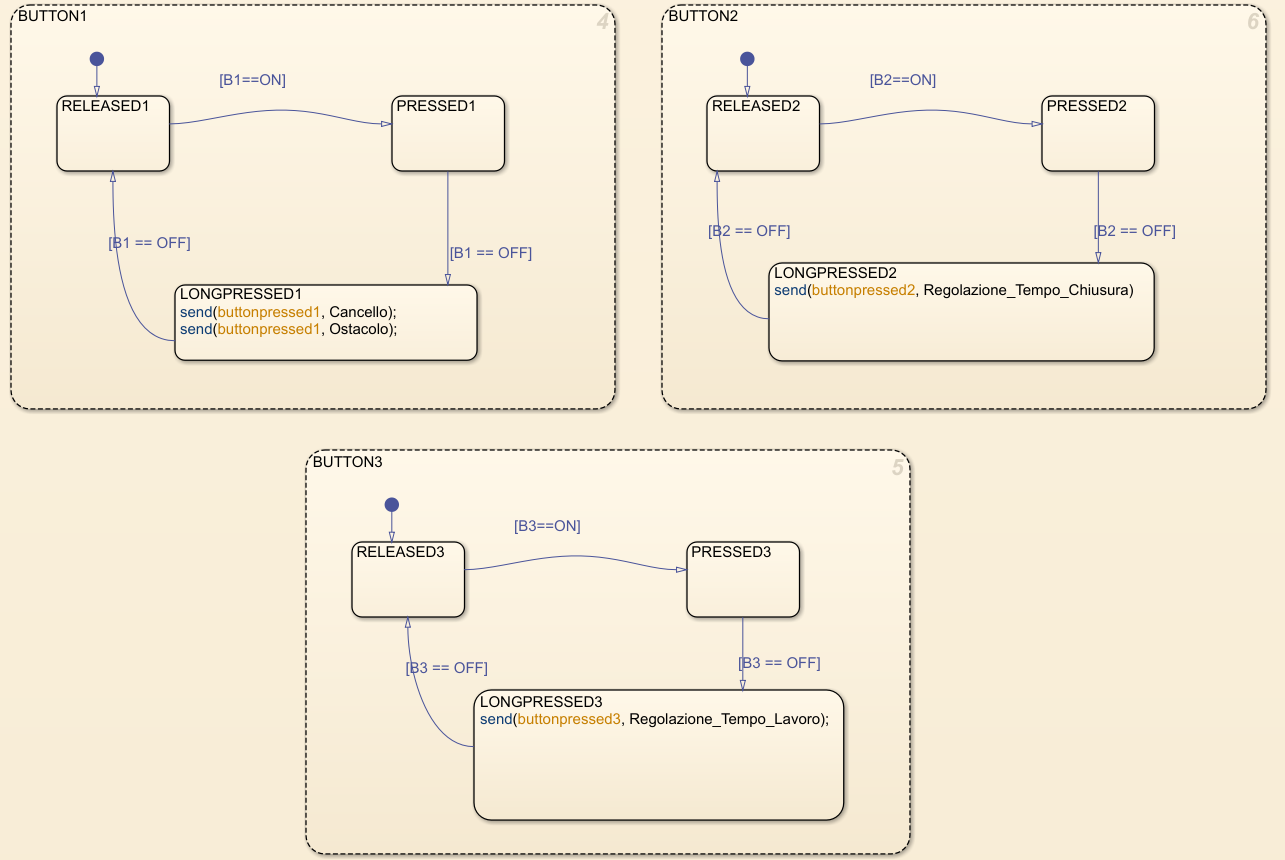
\includegraphics[width=0.9\textwidth]{figures/buttons.png}
                \caption{Stati Buttons}
                \label{buttons}
            \end{figure}

            \noindent \textbf{Button1:}
            \begin{enumerate}
                \item Si entra nello stato \textbf{Released1}, il quale sottolinea il fatto che all'accensione del sistema il pulsante è rilasciato.
                
                \item Alla pressione del pulsante B1 si entra nello stato \textbf{Pressed1}, per segnalare che il pulsante è stato premuto. Questi due stati non presentano azioni in entrata o in uscita, ma sono utilizzati solo per rappresentare l'interazione con l'utente.
                
                \item Quando verrà rilasciato il pulsante, ovvero quando B1 == OFF, si entra nello stato \textbf{Longpressed1}, il quale si occupa di inviare l'evento \textit{buttonpressed1} ai due macrostati \textbf{Cancello} e \textbf{Ostacolo} per segnalare la corretta pressione del pulsante. 
            \end{enumerate}

            \noindent \textbf{Button2 e Button3:}

            \begin{enumerate}
                \item Si entra nello stato \textbf{Released2/Released3}, il quale sottolinea che all'accensione del sistema il pulsante viene rilasciato.
                
                \item Alla pressione del pulsante B2/B3 si entra nello stato \textbf{Pressed2/Pressed3}, per indicare che il pulsante è stato premuto. Questi due stati non posseggono azioni in entrata o in uscita, ma segnalano solo l'interazione con l'utente.
                
                \item Quando verrà rilasciato il pulsante, ovvero quando B2/B3 == OFF, si entra nello stato \textbf{Longpressed2/Longpressed3}, il quale si occupa di inviare l'evento \textit{buttonpressed2/buttonpressed3} ai due macrostati \textbf{Regolazione\_Tempo\_Chiusura} o \textbf{Regolazione\_Tempo\_Lavoro} e segnalarne la corretta pressione. 
            \end{enumerate}

            
    \section{Final Chart}
        \begin{figure}[H]
            \centering
            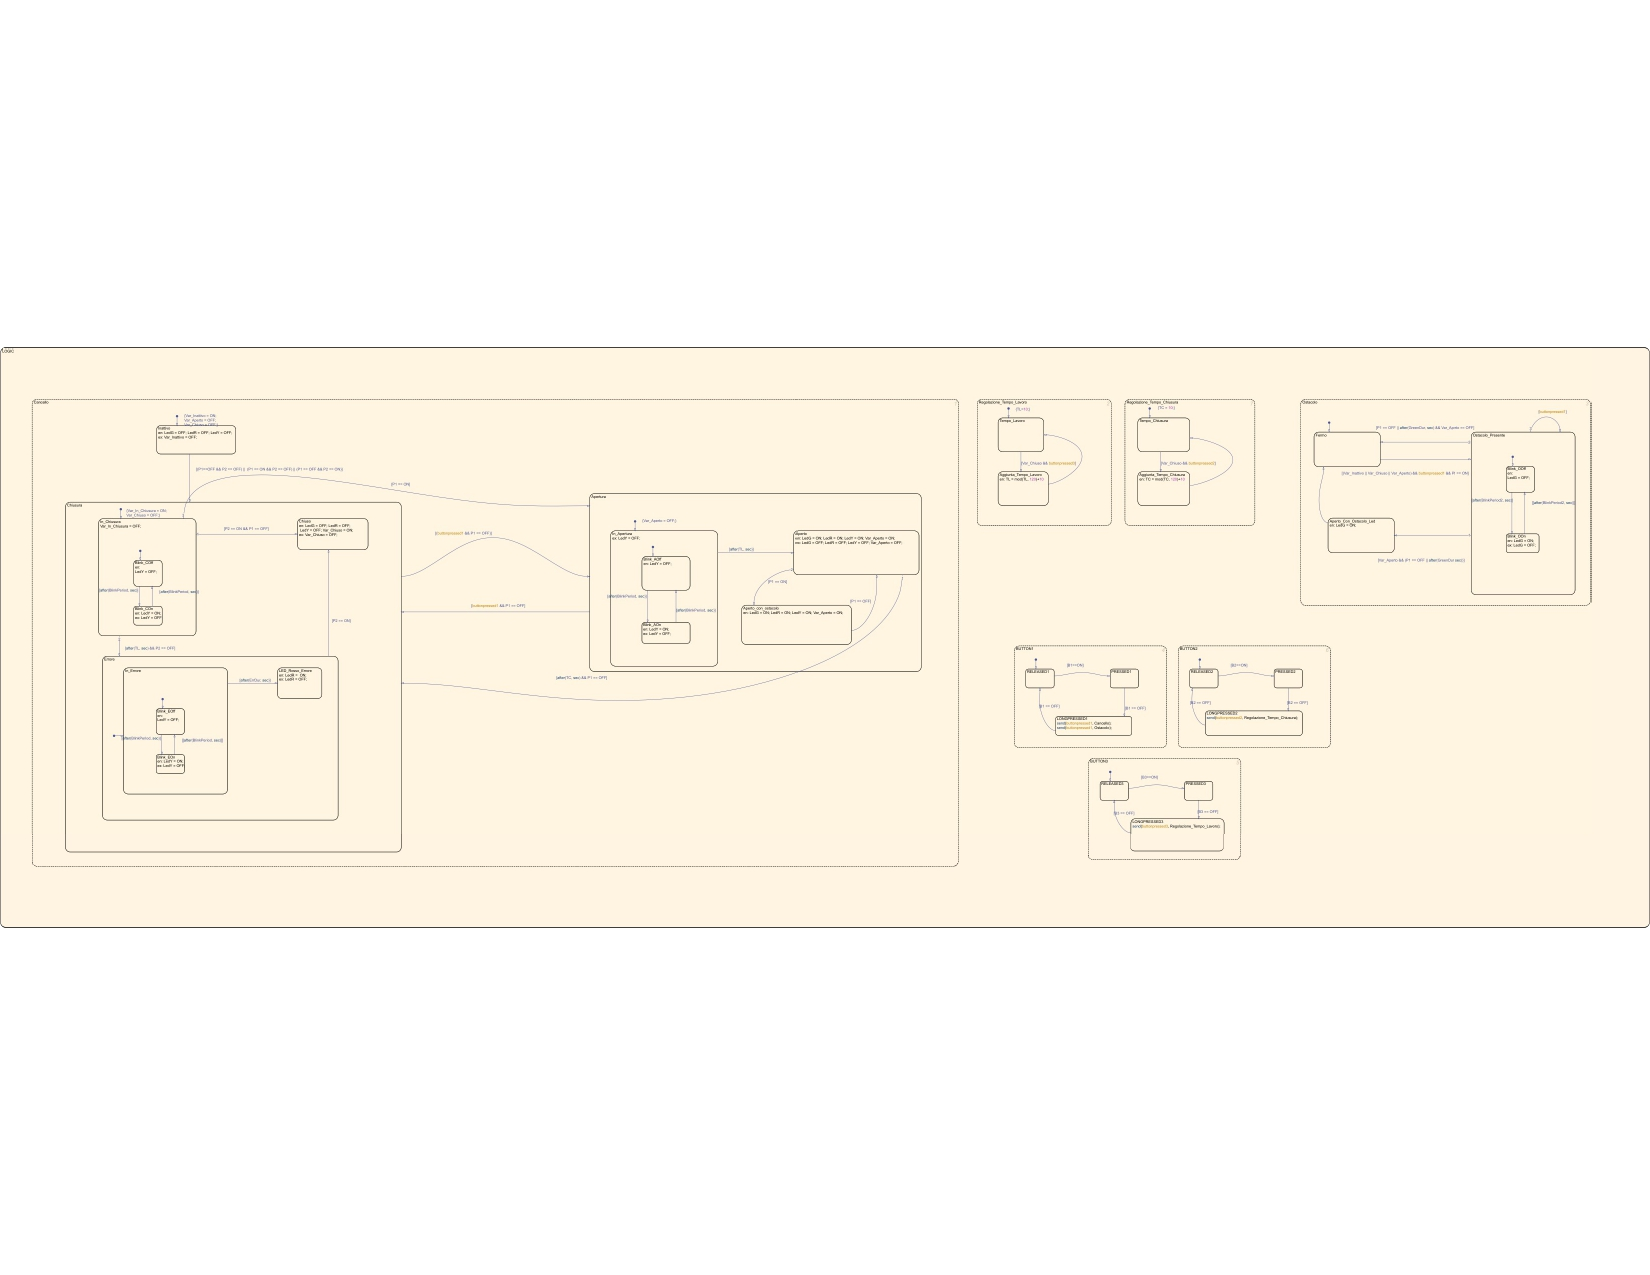
\includegraphics[width=1.5\linewidth, angle=90]{figures/final.jpg}
            \caption{Final Chart}
            \label{final}
        \end{figure}

        Il grafico finale in figura \ref{final} rappresenta il diagramma a stati nella sua interezza. Vi sono 6 macrostati che vengono eseguiti in parallelo grazie alla presenza del macrostato \textbf{LOGIC} esterno avente decomposizione \textbf{AND}.


    \section{Inputs \& Outputs}
        Il grafico in figura \ref{state1} mostra il diagramma precedente con i relativi input e output, ovvero 5 pulsanti (rispettivamente B1, B2, B3, P1, P2) e 3 LED (LedG, LedY, LedR).
        
        \noindent I pulsanti relativi ai sensori di presenza P1 e P2 sono degli switch collegati a delle costanti che vengono poste ad 1 quando il sensore si attiva e a 0 quando il sensore di disattiva.
        Anche i bottoni sono stati collegati a delle costanti ed essi sono configurati in modalità \textit{Momentary}, dunque il loro valore è normalmente 0, ma diventa 1 solo quando viene premuto.
    
        \noindent Per i LED sono stati utilizzati dei blocchi \textit{Out} collegati a blocchi \textit{Lamp} di colore verde, rosso e giallo per segnalarne la corretta accensione.
    
        \begin{figure}[H]
            \centering
            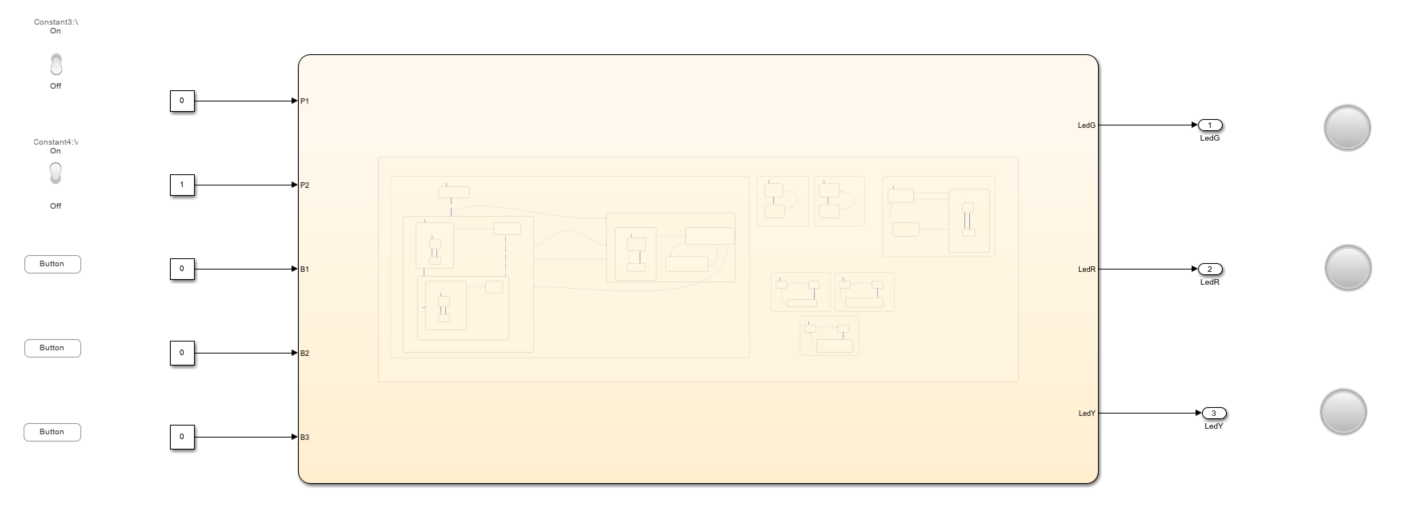
\includegraphics[width=0.9\textwidth]{figures/state.png}
            \caption{Input e Output}
            \label{state1}
        \end{figure}